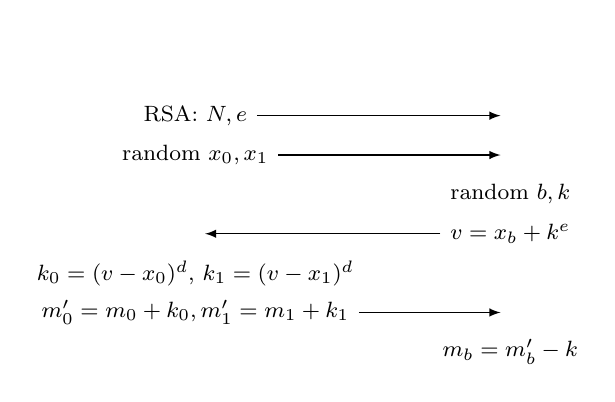
\begin{tikzpicture}[font=\footnotesize]
\node (A) at (0,0) {\Alice};
\node (B) [right of = A, node distance = 4cm] {\Bob};
\node (0a1) [below of=A, node distance=1cm] {RSA: $N,e$};
\node (0b1) [below of=B, node distance=1cm] {};
\draw[-latex] (0a1) -- (0b1) node [midway,above] {};
\node (0a) [below of=0a1, node distance=0.5cm] {random $x_0,x_1$};
\node (0b) [below of=0b1, node distance=0.5cm] {};
\draw[-latex] (0a) -- (0b) node [midway,above] {};
\node (1a) [below of=0a, node distance=0.5cm] {};
\node (1b) [below of=0b, node distance=0.5cm] {random $b, k$};
%\draw[-latex] (1a) -- (1b) node [midway,above] {};
\node (2a) [below of=1a, node distance=0.5cm] {};
\node (2b) [below of=1b, node distance=0.5cm] {$v = x_b+k^e$};
\draw[-latex] (2b) -- (2a) node [midway,above] {};
\node (3a) [below of=2a, node distance=0.5cm] {$k_0 = (v - x_0)^d$, $k_1 = (v - x_1)^d$};
\node (3b) [below of=2b, node distance=0.5cm] {};
%\draw[-latex] (3a) -- (3b) node [midway,above] {};
\node (4a) [below of=3a, node distance=0.5cm] {$m_0'= m_0+k_0, m_1'= m_1+k_1$};
\node (4b) [below of=3b, node distance=0.5cm] {};
\draw[-latex] (4a) -- (4b) node [midway,above] {};
\node (5a) [below of=4a, node distance=0.5cm] {};
\node (5b) [below of=4b, node distance=0.5cm] {$m_b = m_b' - k$};
%\node (6b) [below of=5b, node distance=0.5cm] {Win if $b=b'$};
\end{tikzpicture}
